\section{速度的相对性}\label{sec:02.03}

我们首先讨论质点的直线运动。

取参考系$K$和$K'$的$X$轴都和质点轨迹重合,而两原点$O$、$O'$
相距为$d$(图\ref{fig:02.06})。由式\eqref{eqn:02.02.03}知,$K$,$K'$之间的坐标变换是
    \begin{equation*}
        x'=x-d
    \end{equation*}
现在,若$K'$相对于$K$以均匀速率$u$沿$X$正向运动,则有
    \begin{equation*}
        d=ut+d_0
    \end{equation*}
\vspace{-1.56em}
\begin{figurex}[!h]
    \centering
    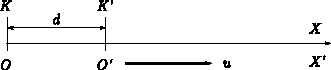
\includegraphics{figure/fig02.06}
    \caption{速度的相对性}
    \label{fig:02.06}
\end{figurex}

\noindent 其中$d_0$是时间$t=0$时,坐标原点$O$,$O'$间的距离。故坐标变换
公式为

~\vspace{-2em}
\begin{equation}
    x'=x-ut-d_0 \label{eqn:02.03.01}
\end{equation}

有了式\eqref{eqn:02.03.01},就不难讨论$K$,$K'$之间的变换关系。

设在$K$系中,质点轨迹函数为
\begin{equation*}
    x=x\left(t\right)
\end{equation*}
根据定义,质点相对于K系的速度为
\begin{equation*}
    v\left(t\right)\equiv\frac{\dif x}{\dif t}
\end{equation*}

相对于$K'$系,由式(2.3.1),质点的轨迹函数应为
\begin{equation*}
    x'=x'\left(t\right)=x\left(t\right)-ut-d_0
\end{equation*}
按照定义,质点相对于$K'$的速度为
\begin{equation*}
    \erratanote{\ensuremath{v\left(t\right)}}{$\left(t\right)$}[][err:02.03.01] \equiv\frac{\dif x'}{\dif t}=\frac{\dif x}{\dif t}-u
\end{equation*}\label{err:02.03.01}
即\vspace{-1.7em}
\begin{equation}
    v'=v-u \label{eqn:02.03.02}
\end{equation}
式\eqref{eqn:02.03.02}就是同一质点相对于$K$及$K'$二者的速度之间的关系。

\begin{wrapfigure}[10]{r}{14.5em}
    \centering
    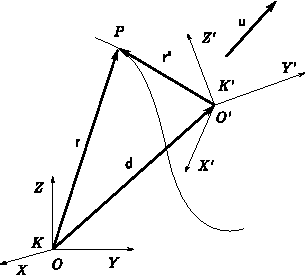
\includegraphics{figure/fig02.07}
    \caption{相对作匀速运动的$K$及$K'$}
    \label{fig:02.07}
\end{wrapfigure}
现在把式\eqref{eqn:02.03.02}推广到三维情况。

由图\ref{fig:02.07}~知,在$K$及$K'$中,质点$P$的位置分别用$\vec{r}$,
$\vec{r'}$表示。它们之间的关系是
{\setlength{\mathindent}{4em}
\begin{equation*}
    \vec{r'}=\vec{r}-\vec{d}
\end{equation*}}%
如果$K'$系相对于$K$系以均匀速度$\vec{u}$运动,则有
{\setlength{\mathindent}{4em}
\begin{equation*}
    \vec{d}=\vec{u}t+\vec{d}_0
\end{equation*}}%
其中$\vec{d}_0$是时刻$t=0$时,从\\$O$到$O'$的矢量。故有
\begin{equation}
    \vec{r}'=\vec{r}-\vec{u}t-\vec{d}_0 \label{eqn:02.03.03}
\end{equation}
若在$K$系中,质点的轨迹函数是
\begin{equation*}
    \vec{r}=\vec{r}\left(t\right)
\end{equation*}
则根据定义,质点相对于$K$的速度是
\begin{equation}\label{eqn:02.03.04}
    \vec{v}\left(t\right)\equiv\frac{\dif \vec{r}}{\dif t}
\end{equation}
另一方面,由式\eqref{eqn:02.03.03}~可以求出质点在$K'$系中的轨迹函数,它是\vspace{-1em}
\begin{equation*}
    \erratanote{\ensuremath{\vec{r}'=}}{$\vec{r}=\dots$}[][err:02.03.02]\vec{r}'\left(t\right)=\vec{r}\left(t\right)-\vec{u}t-\vec{d}_0
\end{equation*}\label{err:02.03.02}
因此,质点相对于$ K' $的速度是
\begin{equation}\label{eqn:02.03.05}
    \vec{v}'\left(t\right)\equiv\frac{\dif \vec{r}'}{\dif t}=\frac{\dif \vec{r}}{\dif t}-\vec{u}
\end{equation}
即\vspace{-2em}
\begin{equation}\label{eqn:02.03.06}
     \vec{v}'=\vec{v}-\vec{u}
\end{equation}
式\eqref{eqn:02.03.06}~就是三维情况的速度变换公式,又称速度合成公式。可
见,在不同参考系中,同一运动可能具有不同速度,亦即速度是
具有相对性的概念。

\begin{wrapfigure}{r}{17em}
    \vspace{-1em}
    \centering
    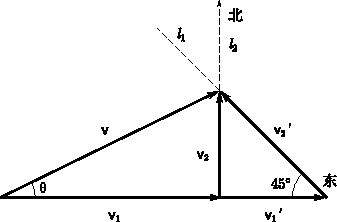
\includegraphics{figure/fig02.08}
    \caption{}
    \label{fig:02.08}
\end{wrapfigure}
\example 一人向东以$v_1=50\text{米/分}$的速度运动,他觉得风从正南
方吹来。假若人行速度增至$v_1'=75\text{米/分}$,他觉得风从东南方吹来。
求风的速度$\vec{v}$。

\solution 设两次感觉到的风速为$\vec{v}_2$和$\vec{v}_2'$。根据题意,各个速度应有以下关系:
\begin{align*}
    \vec{v}_1+\vec{v}_2=\vec{v} \tag{1} \label{xeqn:02.03.01} \\
    \vec{v}_1'+\vec{v}_2'=\vec{v} \tag{2} \label{xeqn:02.03.02}
\end{align*}
作出矢量图(图\ref{fig:02.08})由式\eqref{xeqn:02.03.01}知$\vec{v}$的末端在$l_1$上,由式\eqref{xeqn:02.03.02}知$\vec{v}$的
末端在$l_2$上,故$l_1$和$l_2$的交点是$\vec{v}$的末端。显然有:
\begin{equation*}
        v_1=v_1'-v_1=76-50=25\text{米/分}
\end{equation*}

~\vspace{-1.2em}
\begin{align*}
    v&=\sqrt{v_1^2+v_2^2}=\sqrt{50^2+25^2}=25\sqrt{25}\text{米/分} \\
    \theta&=\arctg\frac{v_2}{v_1}=\arctg\frac{25}{50}=\ang{26;35;}
\end{align*}
从而可看到不同参考系中能感觉到不同的风速。在地球参考系中
风速是$\vec{v}$,以50米/分向东行走的人感觉风速是$\vec{v}_2$;而以75米/分向
东行走的人则感觉到风速是$\vec{v}_2'$。

\example 一列火车以速度$\vec{v}_1$沿水平直轨运行。车上有人以初
速度$\vec{v}_2$竖直向上抛出一小球。车上及地面各站一人研究小球的运
动。在不计空气阻力情况下,不同观察者看到速度,加速度及轨
迹有何不同?

\solution (1)以车为参考系。

因为\vspace{-1em}
\begin{align*}
    &\vec{v}=\vec{v}_x+\vec{v}_y=v_x\vec{i}+v_y\vec{j} \\
    &v_x=0,~ v_y=v_2-gt
\end{align*}
所以\vspace{-1em}
\begin{align*}
    &\vec{v}=\left(v_2-gt\right)\vec{j} \\
    &|\vec{v}|=v_2-gt
\end{align*}
运动在铅直线上进行,是竖直上抛运动;加速度是重力加速度$g$。

(2)以地心为参考系。

因为\vspace{-1em}
\begin{equation*}
    \vec{v}=\vec{v}_x+\vec{v}_y=v_1\vec{i}+\left(v_2-gt\right)\vec{j}
\end{equation*}
故\vspace{-1em}
\begin{equation*}
        |\vec{v}|=v=\sqrt{v_1^2+\left(v_2-gt\right)^2}
\end{equation*}
这表示速度的大小、方向都在变。运动方程是
\begin{equation*}
    \left\{\begin{array}{l}
        x=v_1t \\
        y=v_2t-\dfrac{1}{2}gt^2
    \end{array}\right.
\end{equation*}
轨道方程为抛物线
\begin{equation*}
    y=\frac{v_2}{v_1}x-\frac{g}{2v_1}x^2
\end{equation*}

\noindent 加速度$\vec{a}=\dfrac{\dif \vec{v}}{\dif t}=-g\vec{j}$,沿垂直方向向下。

(3)以地面为参考系,小球沿抛物线运动,相当于一个以初速
率$\displaystyle v_0=\sqrt{v_1^2+v_2^2}$,抛射角为$\theta=\arctg\dfrac{v_2}{v_1}$的抛射体运动。

\begin{wrapfigure}[9]{r}{12em}
    \vspace{1em}
    \centering
    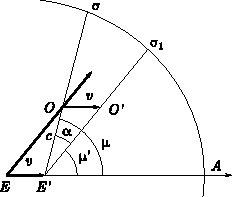
\includegraphics{figure/fig02.09}
    \caption{}
    \label{fig:02.09}
\end{wrapfigure}
\example 光行差现象。

具有不同运动状态的观察者所见的星体的方位是不同的,这
种差别叫做光行差。因地球公转运动而产生的光行差称为周年光
行差,因地球自转而产生的光行差称为周日光行差。

在图\ref{fig:02.09}~中,若观测者相对于某星是静止的,他观测到某星
在天球上的位置是$\sigma$,则星光到达望远镜物镜中心$O$时,其目镜位
置在$E'$点。若观测者跟随着地球运动,$EE'$为此时地球的运动方
向,因星光由$O$点到达目镜的时间为$\tau$,故在此时间内,地球运
行的距离为$EE'=\tau v$($\vec{v}$为地球运动的速度);因光速为$c$,当星
光到达目镜时,目镜已移至$E'$点,所以$OE'=\tau c$是星光在$\tau$内传
播的距离。若地球静止不动,则望远镜对准基的方向为$E'O$。当
地球运动时,望远镜指向$E'O'$方向才能接收到星光,这是星的视
方位。相应的,星由真位置$\sigma$移至视位置$\sigma_1$,

设星的真方位与观测者速度$\vec{v}$间的交角为\erratanote{$\mu$}{$u$}[疑“$\mu$”误作“$u$”。],星的视方位与
$\vec{v}$的夹角为$\mu'$,则光行差为$\alpha$,且有
\begin{equation*}
    \alpha=\mu-\mu'
\end{equation*}
由三角形$OO'E'$,得
\begin{equation*}
    \frac{\sin\alpha}{\sin\mu'}=\frac{OO'}{OE'}=\frac{\tau v}{\tau c}=\frac{v}{c}
\end{equation*}

\begin{equation*}
    \sin\alpha=\frac{v}{c}\sin\mu'
\end{equation*}
因为$\alpha$很小,所以
\begin{align*}
    \alpha&\approx\frac{v}{c}\sin\mu'\text{弧度} \\
        &=\frac{v}{c}\sin\mu'\times\frac{180}{\uppi}\times 60 \times 60 \text{秒} \\
        &=\frac{v}{c}\sin\mu'\times 206265\text{秒} \\
        &=k\sin\mu'\text{秒}
\end{align*}
其中$k$称为光行差常数。

已知地球公转速率为$v=29.770\text{公里/秒}$,光速$c=299,774
\text{公里/秒}$,所以周年光行差常数
\begin{equation*}
    k_\text{年}=\frac{29.770}{299,774}\times 206,265=20.48\text{秒}
\end{equation*}

已知地球半径$R=6,378\text{公里}$。地球自转一周的时间为$T=
86,164\text{秒}$。所以在纬度$\varphi$处的地面速度为
\begin{equation*}
    v_\varphi=\frac{2\uppi R\cos\varphi}{T}=0.464\cos\varphi\text{公里/秒}
\end{equation*}
因此,周日光行差常数为
\begin{align*}
    k_\varphi&=\frac{0.464}{299,774}\times 206,265\times\cos\varphi\text{秒} \\
        &=0.32\cos\varphi\text{秒}
\end{align*}